\chapter{Глава 1 Логическое рассуждение}

Выделение целой главы такой стратегии, как логическое рассуждение, может показаться излишним. В самом деле, без логического мышления, хотя оно и ислользуется для решения задач, немыслимо применение ни одной стратегии. Для многих людей решение задач является практически синонимом логического рассуждения, или логического мышления. Так зачем же тогда нужна эта глава, и зачем вообще выделять эту стратегию?

В повседневной жизни мы приостасем R JIULMHECLRUMY раст суждению, когда спорим о чем-нибудь с кем-то. И это понятно — во время спора мы рассчитываем на то, что определенные доводы будут вызывать конкретную реакцию. На работе мы с помощью логической цепочки доводов добиваемся изменения того или иного производственного процесса. Мы логически выстраиваем цепочку утверждений в надежде на получение желаемого вывода. В суде, например, адвокаты используют логическое рассуждение, чтобы представить дело в нужном им свете. Если мы назначаем кому-то встречу через два дня, а сегодня суббота, то логика подсказывает нам, что встреча должна состояться B понедельник.

В математике некоторые задачи решаются без использования каких-либо других стратегий, включая и представленные в этой книге. Они требуют строгих рассужде. ний и формулирования утверждений, которые логически вытекают одно M3 другого. Возьмем, например, такую задачу.

Найдите все пары простых чисел, сумма которых равна 741.

Многие наверняка составят перечень всех простых чи- меньше 741 и будут подбирать к ним пару, дающую в сумме 741. Вместе с тем работу можно упростить с помощью логического рассуждения. Если сумма двух чисел является нечетным числом, то одно из слагаемых должно быть нечетным, а другое — четным. Как известно, существует только одно четное простое число — 2. Значит, другим числом должно быть 739 (а 739 — это простое число). Таким образом, мы нашли все пары, которые удовлетвосел ряют условиям задачи.

Рассмотрим еще одну задачу, которая решается путем логического рассуждения.

‘Залиндромическим называют такое число, которое чи- тается одинаково слева направо и справа налево. При- мерами трехзначного и четырехзначного палиндромов являются 373 и 8668. Мария выписала все трехзначные палиндромы на листочки бумаги и положила их в большую коробку. Мигель выписал все четырехзначные палиндромы и положил листочки с числами в ту же коробку. Учитель тщательно перемешал листочки и попросил Лору B3ATb один из них He глядя. Какова вероятность того, что она вытащит четырехзначный палиндром?

окажется красным, то в этой коробке на самом деле нахо- дятся только красные бантики, поскольку они не разно- цветные. Пометим ее как «Красные». Коробка с ярлыком «Белые» не может содержать чисто белые бантики, поэтому она должна получить ярлык «Разноцветные». Наконец, на коробку, ошибочно помеченную как «Красные», нужно наклеить ярлык «Белые». РР

Обратите внимание на TO, что для решения каждой из рассмотренных задач необходимы всего лишь логическое рассуждение и размышление. Это ни B коей мере не 03начает, что логическое мышление не требуется при использовании других стратегий решения задач, однако задачи, представленные в этой главе, решаются ПОЧТИ ИСКЛЮЧИ- тельно путем логического рассуждения.

\section{ЗАДАЧА 1.1}

Макс начинает отсчитывать натуральные числа в порядке увеличения: 1, 2, 3, 4, ..., а Сэм ведет отсчет с той же скоростью, HO в обратном порядке от числах: X, X — 1,х-2,х-3, х-4, ... Когда Макс доходит до 52, Сэм называет число 74. С какого числа (x) Сэм начал обратный отсчет?

\section{Обычный подход}

Столкнувшись с такой задачей, большинство людей обычно пытаются воспроизвести описанную ситуацию, T. €. выпол- нить одновременно процедуры отсчета, чтобы посмотреть, какой получится результат. Сложность здесь, однако, заключается в TOM, что начальное число для обратного отсчета неизвестно, поэтому, скорее всего, будут использоваться ПРЯМОЙ отсчет и метод последовательного ПРИбЛИЖСНИЯ. Это не TONTRKO TONTO WO я OUALIL лл

\section{образцовое решение}

Подойдем к решению задачи логически. Макс отсчитал 52 числа, а значит и Сэм отсчитал такое же количество чисел. Можно представить 52-е число Сэма какх - 51. Как известно, это число равно 74. Таким образом, мы получаем уравнение х - 51 = 74, из которого следует, что х = 125.

\section{ЗАДАЧА 1.2}

У нас 100 кг свежих ягод, в которых 99\% массы приходится на воду. Через некоторое время содержание воды в ягодах уменьшается до 98\%. Сколько теперь весят ягоды?

\section{Обычный подход}

Чаще всего говорят, что после испарения 1\% воды вес ягод должен уменьшиться до 99\%, а значит ягоды весят 99 кг. Это неправильно!

\section{Образцовое решение}

Попробуем найти ответ путем логического рассуждения. Исходно в ягодах содержится 99\% воды, т.е. в них 99 кг воды и 1 кг сухого вещества, иначе говоря, масса сухих ягод составляет 1\%. Масса сухого вещества не меняется: в конце процесса сушки она так и останется равной 1 кг. Вместе стем доля того, что не является водой, удваивается до 2\%.

Для того, чтобы нечто, имеющее фиксированное количе- ство (1 кг сухого вещества в нашем случае), удвоило свою долю (с 1\% до 2\%), суммарное количество смеси должно уменьшиться в два раза. В начале у нас был 1\% сухого веще- ства, ил На 2 1 и И 100° 2B конце — 2\%, или 700° что сокращает

до \%’ T.€. мы получаем 1 кг сухого вещества в 50 кг сум- марной массы. Таким образом, в конце B ягодах остается 49 кг воды.

\section{ЗАДАЧА 1.3}

Во время школьного эксперимента Мигель многократно бросает обычный шестигранный игральный кубик. Он следит за каждой выпавшей цифрой и хочет остановиться, как только одна цифра выпадет три раза. Мигель останавливается после 12-ro 6pocka, и сумма выпавших цифр составляет 47. Какая цифра выпала третий раз? (Обычный шестигранный игральный кубик имеет цифры от 1 до 6.)

\section{Обычный подход}

Одно из решений — это взять игральный кубик и поэкспериментировать с ним. Получить точно 47 очков за 12 бросков довольно трудно, но даже если это и получится, то такое решение нельзя назвать изящным!

\section{Образцовое решение}

Давайте порассуждаем. За 11 бросков ни одна цифра He выпала три раза, иначе эксперимент закончился бы. Это означает, что пять цифр выпали дважды, а одна — лишь однократно. Обозначим эту цифру символом М. Если М выпадет в 12-м броске, то сумма будет равна 2 (1 + 2 + 3 + 4 + 5 + 6) = 42. Таким образом, сумма после 11 бросков составляет 42 — М. Если № — число, выпавшее B третий pa3, то 42 - М + N = 47, а№-М = 5. Мы 3HaeM, что МиМ могут иметь значения только от 1 до 6. Единственные

два числа из данного ряда, которые имеют разность 5, это 6 1 1. С учетом такого ограничения уравнение N - M = 5 имеет единственное решение, где M = 1, a N = 6. Таким образом, в третий раз выпала цифра 6.

\section{ЗАДАЧА 1.4}

Имеется треугольник, периметр которого численно равен его площади. Чему равен радиус вписанной в треугольник окружности?

\section{Обычный подход}

Обычно при решении этой задачи строят чертеж, как показано на рис. 1.1, и подбирают значения в попытке найти ответ. При таком подходе нужно быть готовым к разочарованиям.


\begin{figure}[!h]
\centering
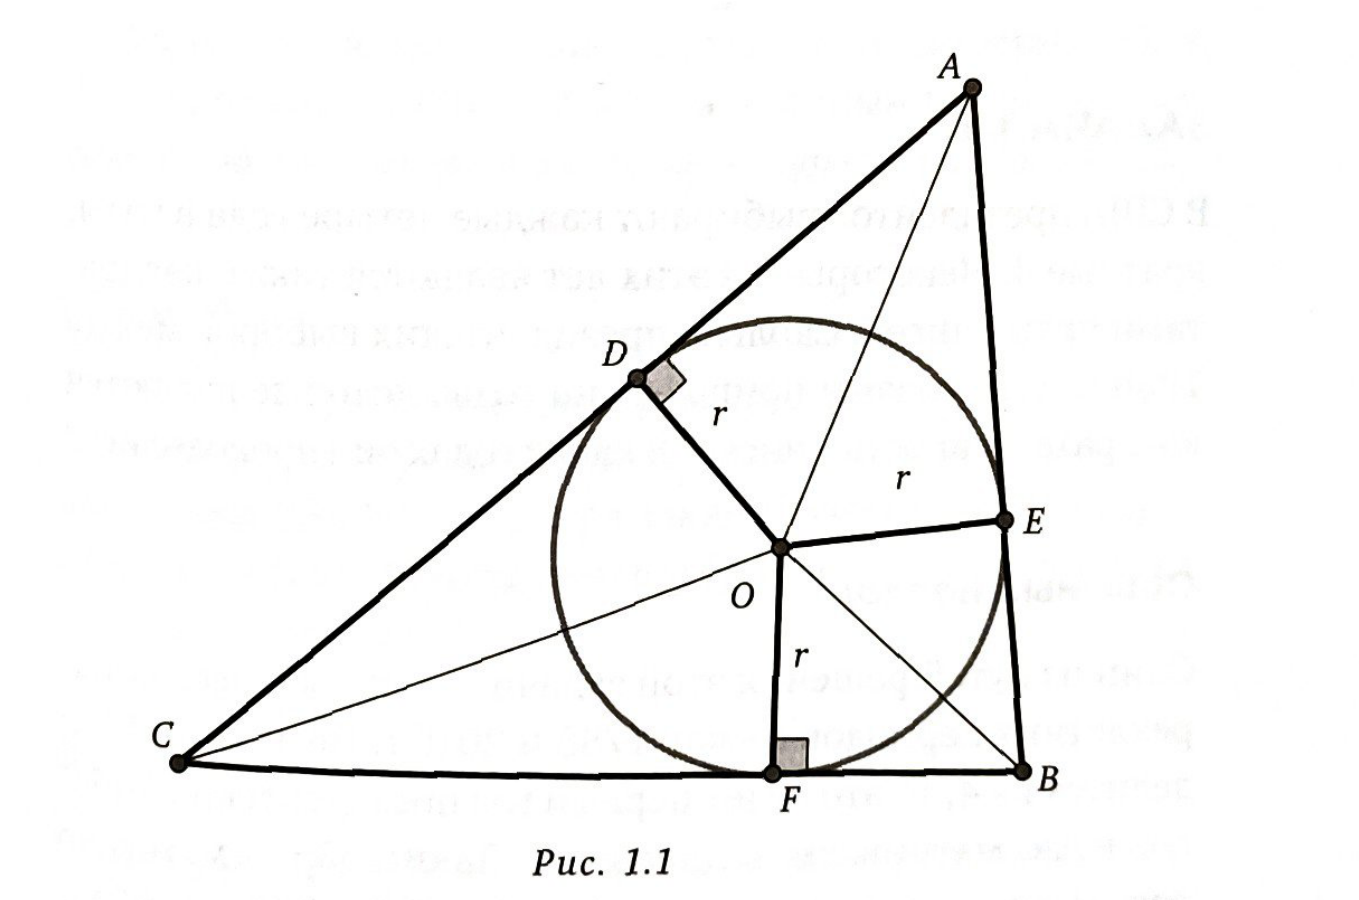
\includegraphics[width=10cm, height=6.622516556291391cm]{/home/f/Programming/projects/scans\_to\_pdf\_cg\_cv/latex/result\_here/files/img1.png}
\caption{}
\end{figure}
        

\section{Образцовое решение}

Для решения этой задачи необходимо немного логики и следование поставленным условиям. Начнем с треугольника ABC, периметр которого равен p = АВ + ВС + СА. Обозначим символом О центр вписанной окружности с радиусом г. Площадь треугольника АВС равна сумме площадей треугольников АОВ, ВОС и СОА с основаниями АВ, ВС и СА, соответственно, и высотой г. Это дает нам следующее урав- нение:


\begin{figure}[!h]
\centering
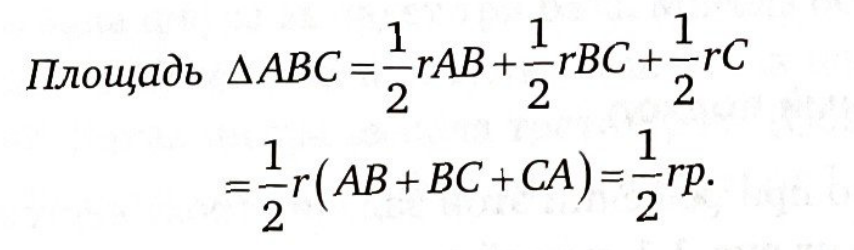
\includegraphics[width=10cm, height=2.927400468384075cm]{/home/f/Programming/projects/scans\_to\_pdf\_cg\_cv/latex/result\_here/files/img2.png}
\caption{}
\end{figure}
        

Поскольку периметр треугольника численно равен его 1 площади, мы получаем: Егр =pur=2.

\section{ЗАДАЧА 1.5}

B США президентов выбирают каждые четыре года B годы, кратные 4. Некоторые U3 этих лет являются также квадратами целых чисел. Сколько президентских выборов между 1788 и 2016 годами пришлось на годы, которые ЯВЛЯЮТСЯ квадратами простых чисел? В каких годах они проводились?

\section{Обычный подход}

Один из путей решения этой задачи — перебор всех че15” рехлетних периодов между 1788 и 2016 г. Поскольку 1788 делится на 4, то это будет первый год президентских выборов в рассматриваемом диапазоне. Таким образом, можно составить перечень этих лет (1788, 1792, 1796, ..., 2012,

